\documentclass[tikz]{standalone}
\usepackage{standalone}
%\usetikzlibrary{arrows.meta, decorations.pathreplacing, shapes.geometric}
\usetikzlibrary{bayesnet}

\begin{document}

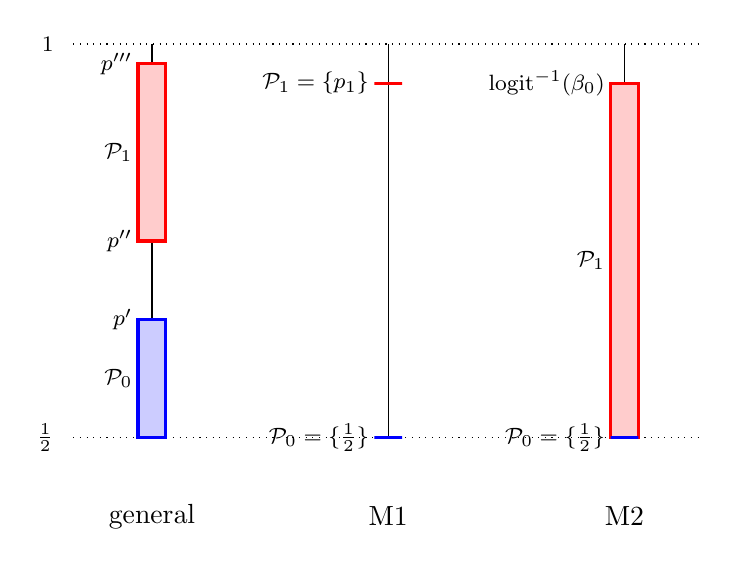
\begin{tikzpicture}[thin]

\draw[dotted, thin, yshift=5 cm] (-1,0) node[label=left:1] (one) {} -- (7,0);
\draw[dotted, thin] (-1,0) node[label=left:\(\frac{1}{2}\)] (half) {} -- (7,0);

\node (a) at (0,-1) {general};
\node (b) at (3,-1) {M1};
\node (c) at (6,-1) {M2};

\draw
(a|-half) --
node[pos=0.15, label=left:{\(\mathcal{P}_0\)}] (a-P0) {}
node[pos=0.3, label=left:{\(p'\)}] (a-P0-r) {}
node[pos=0.5, label=left:{\(p''\)}] (a-P1-l) {}
node[pos=0.725, label=left:{\(\mathcal{P}_1\)}] (a-P1) {}
node[pos=0.95, label=left:{\(p'''\)}] (a-P1-r) {}
(a|-one)
(b|-half) --
node[pos=0, label=left:{\(\mathcal{P}_0=\{\frac{1}{2}\}\)}] (b-P0-r) {}
node[pos=0.9, label=left:{\(\mathcal{P}_1=\{p_1\}\)}] (b-P1-l) {}
(b|-one)
(c|-half) --
node[pos=0, label=left:{\(\mathcal{P}_0=\{\frac{1}{2}\}\)}] (c-P0-r) {}
node[pos=0.45, label=left:{\(\mathcal{P}_1\)}] (c-P1) {}
node[pos=0.9, label=left:{\(\mathrm{logit}^{-1}(\beta_0)\)}] (c-P1-l) {}
(c|-one)
;

% general
\draw[very thick, red, fill=red!20] ([xshift=-5] a-P1-r) rectangle ([xshift=5] a-P1-l);
\draw[very thick, blue, fill=blue!20] ([xshift=-5] a|-half) rectangle ([xshift=5] a-P0-r);

% M1
\draw[very thick, red, fill=red!20] ([xshift=-5] b-P1-l) rectangle ([xshift=5] b-P1-l);
\draw[very thick, blue, fill=blue!20] ([xshift=-5] b|-half) rectangle ([xshift=5] b-P0-r);

% M2
\draw[very thick, red, fill=red!20] ([xshift=-5] c|-half) rectangle ([xshift=5] c-P1-l);
\draw[very thick, blue, fill=blue!20] ([xshift=-5] c|-half) rectangle ([xshift=5] c-P0-r);

\end{tikzpicture}

\end{document}
